\title{\textbf{GoldFinch-AHN: Adaptive Hybrid Network with Sliding-Window Attention and Learnable Preservation Gate}

\author{Anonymous authors}



\section{Introduction}

\subsection{Motivation}

Hybrid attention architectures combine multiple attention mechanisms with 
the goal of capturing both short-range and long-range dependencies 
efficiently. A common pattern is:

\[
\text{Output} = g \cdot \text{Local}(X) + (1 - g) \cdot \text{Global}(X)
\tag{1.1}
\]

where $g$ is a mixing coefficient. The rationale: local attention captures 
fine-grained context at low cost, while global attention captures long-range 
semantics.

The \textbf{challenge} is twofold:

\begin{enumerate}
\item \textbf{Mixing the two branches correctly.} A fixed $g$ (e.g., $0.5$) ignores
  that different tokens have different local/global needs.
\item \textbf{Preserving pretrained behavior.} Replacing attention with a new
  mechanism risks breaking the residual stream that downstream layers
  depend on.

\end{enumerate}
\subsection{Our Approach}

\textbf{GoldFinch-AHN} addresses both:

\begin{enumerate}
\item \textbf{Input-dependent gating.} Per-token gate $g_t = \sigma(W_g x_t)$
  determines how much each token relies on local vs. global.
\item \textbf{Preservation gate.} A block-level residual with learnable coefficient:
  $$
  Y = \alpha \cdot \text{Block}(X) + (1 - \alpha) \cdot X
  \tag{1.2}
  $$
  with $\alpha = \sigma(2.0) \approx 0.88$ at initialization.

\end{enumerate}
\subsection{Honest Disclosures}

Two implementation details must be disclosed before the methodology:

\textbf{The "long-memory" branch is a linear projection.} In the code, the class 
\texttt{GatedDeltaNetLayer} is:

\begin{lstlisting}
class GatedDeltaNetLayer(nn.Module):
    def __init__(self, d_model, use_spectral_norm=False):
        super().__init__()
        self.net = nn.Linear(d_model, d_model)

    def forward(self, x):
        return self.net(x)
\end{lstlisting}

There is no recurrence, no state update, no delta rule. It is a single 
\texttt{nn.Linear}. In our experiments this branch is essentially a 
content-independent projection.

\textbf{The preservation gate is a residual connection.} The \texttt{output\_gate} 
parameter blends the block's output with the block's input -- a learnable 
residual. It is not an attention mechanism.

We include these disclosures to enable fair evaluation: GoldFinch-AHN 
should be compared against other attention-replacement methods with the 
understanding that it is more conservative than they are.

\subsection{Contributions}

\begin{itemize}
\item \textbf{A hybrid attention block} with sliding-window attention, an input-dependent
  gate, and a preservation gate.
\item \textbf{An empirical evaluation} on DistilBERT, RoBERTa, and GPT-2 on SST-2.
\item \textbf{Honest implementation disclosure}: the long-memory branch is a linear
  projection, not a recurrent mechanism.
\item \textbf{Full reproducibility}, including code and checkpoints.

\end{itemize}
\subsection{Paper Organization}

Section 2 reviews hybrid attention, sliding-window mechanisms, and residual 
gating. Section 3 provides background on attention, gating, and residuals. 
Section 4 presents GoldFinch-AHN. Section 5 covers integration. Section 6 
details the setup. Section 7 reports results. Section 8 analyzes the 
mechanism. Section 9 discusses. Section 10 lists limitations. Section 11 
concludes.



\subsection{Notation}

\begin{table}[H]
\centering
\small
\begin{tabular}{lll}
\toprule
\textbf{Symbol} & \textbf{Meaning} & \textbf{First appears} \\
\midrule
$X$ & Input hidden states & 1.1 \\
$g$ & Mixing gate & 1.1 \\
$\alpha$ & Preservation coefficient & 1.2 \\
$W$ & Window size & 3.2 \\
$d$ & Hidden size & 3.1 \\
$H$ & Number of heads & 3.1 \\
$r$ & LoRA rank & 4.4 \\
\bottomrule
\end{tabular}
\end{table}
</parameter>




\section{Related Work}

\subsection{Hybrid Attention}

\textbf{Longformer} (Beltagy et al., 2020). Sliding-window + global tokens. 
Longformer's window is fixed; ours is token-adaptive via a gate.

\textbf{BigBird} (Zaheer et al., 2020). Sliding-window + random + global. 
Theoretically universal.

\textbf{Hybrid Transformer} (Zhu et al., 2021). Local attention + low-rank 
global. Similar in spirit.

\textbf{Our approach.} Sliding-window + linear projection + preservation gate.

\subsection{Sliding-Window Attention}

\textbf{Longformer} (Beltagy et al., 2020). The canonical sliding-window 
implementation.

\textbf{Mistral} (Jiang et al., 2023). Uses sliding window for efficiency.

\textbf{Our approach.} Sliding-window with an input-dependent gate.

\subsection{Residual and Preservation}

\textbf{LayerScale} (Touvron et al., 2021). Multiplies residual branch by small 
learnable scalar.

\textbf{ReZero} (Bachlechner et al., 2021). Zero-initialized residual branch 
with learnable scalar. Ensures identity at initialization.

\textbf{Our approach.} Preservation gate blends output with input via learnable 
$\alpha = \sigma(2.0) \approx 0.88$. Similar to ReZero but with a 
non-zero initialization.

\subsection{Linear Attention and State-Space}

\textbf{Linear Transformer} (Katharopoulos et al., 2020). Linear attention.

\textbf{Gated DeltaNet} (Yang et al., 2024). Delta-rule recurrent.

\textbf{Note.} Our long-memory branch is a \textbf{linear projection}, not a recurrent 
mechanism. See Section 1.3.

\subsection{Position of Our Work}

\begin{table}[H]
\centering
\small
\begin{tabular}{lll}
\toprule
\textbf{Axis} & \textbf{Prior work} & \textbf{Ours} \\
\midrule
\textbf{Local attention} & Sliding window & Sliding window \\
\textbf{Long memory} & Recurrent & \textbf{Linear projection} \\
\textbf{Mixing} & Fixed or gate & Input-dependent gate \\
\textbf{Preservation} & LayerScale, ReZero & Preservation gate \\
\bottomrule
\end{tabular}
\end{table}

\textbf{Key distinction.} GoldFinch-AHN is \textbf{conservative}: the preservation 
gate keeps the block close to identity. This reduces risk but also reduces 
potential gains.



\subsection{Comparison Table}

\begin{table}[H]
\centering
\small
\begin{tabular}{lllll}
\toprule
\textbf{Method} & \textbf{Local} & \textbf{Long} & \textbf{Gate} & \textbf{Preserve} \\
\midrule
Longformer & Window & Global tokens & Fixed & No \\
BigBird & Window & Random + global & Fixed & No \\
ReZero & N/A & N/A & N/A & Yes \\
LayerScale & N/A & N/A & N/A & Yes \\
\textbf{GoldFinch-AHN} & \textbf{Window} & \textbf{Linear} & \textbf{Input} & \textbf{Yes} \\
\bottomrule
\end{tabular}
\end{table}




\section{Background}

\subsection{Multi-Head Attention}

Standard attention:

\[
\text{Attn}(Q, K, V) = \text{softmax}\!\left(\frac{QK^\top}{\sqrt{d}}\right)V
\tag{3.1}
\]

\subsection{Sliding-Window Attention}

A sliding-window mask restricts attention to nearby tokens:

\[
M_{ij} = \begin{cases} 1 & |i - j| \leq W/2 \\ 0 & \text{otherwise} \end{cases}
\tag{3.2}
\]

Then:

\[
\text{Attn}_\text{window}(Q, K, V) = \text{softmax}\!\left(\frac{QK^\top}{\sqrt{d}} + \log M\right)V
\tag{3.3}
\]

\textbf{Complexity.} $\mathcal{O}(L W)$ time, $\mathcal{O}(L W)$ memory. Linear 
in $L$ for fixed $W$.

\subsection{Gating}

An input-dependent gate:

\[
g_t = \sigma(W_g x_t + b_g)
\tag{3.4}
\]

where $W_g \in \mathbb{R}^{d \times k}$ and $k$ is the gate dimension. 
The gate can be per-token, per-head, or scalar.

\textbf{Initialization.} Bias $b_g$ controls the initial gate value. Common choices:
\begin{itemize}
\item $b_g = 0$: $\sigma(0) = 0.5$ (equal mixture)
\item $b_g = 2$: $\sigma(2) \approx 0.88$ (favor first branch)
\item $b_g = -2$: $\sigma(-2) \approx 0.12$ (favor second branch)

\end{itemize}
\subsection{Preservation Gate (Residual with Learnable Coefficient)}

A preservation gate blends the block output with the block input:

\[
Y = \alpha \cdot F(X) + (1 - \alpha) \cdot X
\tag{3.5}
\]

where $\alpha = \sigma(W_\alpha)$ is learnable.

\textbf{Special cases:}
\begin{itemize}
\item $\alpha = 1$: pure residual (standard transformer)
\item $\alpha = 0$: pure identity (block ignored)
\item $\alpha = 0.5$: half residual

\end{itemize}
\textbf{ReZero} (Bachlechner et al., 2021). Uses $\alpha = 0$ at initialization, 
i.e., identity at start. Our choice of $\alpha = \sigma(2) \approx 0.88$ is 
different: we start with residual-dominant but not identity.

\subsection{LoRA}

LoRA (Hu et al., 2021):

\[
W_\text{eff} = W_\text{frozen} + \frac{\alpha_L}{r} BA
\tag{3.6}
\]

with $B = 0$ at initialization.

\subsection{Notation Summary}

\begin{table}[H]
\centering
\small
\begin{tabular}{ll}
\toprule
\textbf{Symbol} & \textbf{Meaning} \\
\midrule
$L$ & Sequence length \\
$d$ & Hidden size \\
$H$ & Number of heads \\
$W$ & Window size \\
$g$ & Mixing gate \\
$\alpha$ & Preservation coefficient \\
$r$ & LoRA rank \\
\bottomrule
\end{tabular}
\end{table}
</parameter>




\section{Method}

\subsection{Overview}

GoldFinch-AHN has the following structure:

\begin{lstlisting}
                    Input X
                       |
        +--------------+--------------+
        |              |              |
                                       
    +------+       +------+      +-----------+
    |  Q   |       |  K   |      |  Linear   |
    | proj |       | proj |      |  (delta)  |
    +--+---+       +--+---+      +-----+-----+
       |              |                |
                                        
   +----------------------+      +-----------+
   | Sliding-window       |      | long_out  |
   | attention            |      +-----+-----+
   +--------+-------------+            |
            | short_out                |
            |                          |
       +----+--------------------------+----+
       |                                    |
       |  gate(x) $\to$ per-token mixing        |
       |  fused = g * short + (1-g) * long  |
       +--------+---------------------------+
                |
                 
       +------------------+
       | out_proj         |
       +--------+---------+
                |
                 
       +------------------+
       | Preservation     |
       | gate: $\alpha$ out +    |
       | (1-$\alpha$) x          |
       +--------+---------+
                |
                 
              Output
\end{lstlisting}

\subsection{Sliding-Window Attention}

We compute standard scaled dot-product attention with a band mask:

\[
\text{scores}_{ij} = \frac{q_i^\top k_j}{\sqrt{d}}
\tag{4.1}
\]

Apply window mask:

\[
M_{ij} = \begin{cases} 1 & |i - j| \leq W \\ 0 & \text{otherwise} \end{cases}
\tag{4.2}
\]

For causal decoders:

\[
M_{ij} = \begin{cases} 1 & 0 \leq i - j \leq W \\ 0 & \text{otherwise} \end{cases}
\tag{4.3}
\]

Then:

\[
\text{short}_i = \sum_j \text{softmax}_j(\text{scores}_{ij} + \log M_{ij}) v_j
\tag{4.4}
\]

\subsection{Long-Memory Branch (Linear Projection)}

\textbf{Important.} The code refers to this as \texttt{GatedDeltaNetLayer} but 
implements:

\begin{lstlisting}
long_out = self.delta_mem(x)  # = Linear(x)
\end{lstlisting}

There is no recurrence, no gating, no state. It is a single linear 
projection $W_m \in \mathbb{R}^{d \times d}$. Its role in the architecture 
is:

\[
\text{long}_t = W_m x_t + b_m
\tag{4.5}
\]

\textbf{Interpretation.} The long-memory branch is a per-token learned 
transformation. It cannot capture long-range dependencies because it 
processes each token independently.

\subsection{Input-Dependent Gate}

The gate:

\[
g_t = \sigma(W_g x_t + b_g) \in \mathbb{R}^H
\tag{4.6}
\]

with $W_g \in \mathbb{R}^{d \times H}$ and $b_g \in \mathbb{R}^H$.

\textbf{Mean over heads:} In forward, the gate is reduced to a scalar per token:

\[
g'_t = \frac{1}{H} \sum_{h=1}^H g_{t,h}
\tag{4.7}
\]

\textbf{Fusion:}

\[
\text{fused}_t = g'_t \cdot \text{short}_t + (1 - g'_t) \cdot \text{long}_t
\tag{4.8}
\]

\subsection{Output Projection and Preservation Gate}

Output projection:

\[
\text{out} = W_O \cdot \text{fused} + b_O
\tag{4.9}
\]

Then the preservation gate:

\[
\alpha = \sigma(w_\alpha) \approx 0.88 \text{ at init}
\tag{4.10}
\]

\[
Y = \alpha \cdot \text{out} + (1 - \alpha) \cdot x
\tag{4.11}
\]

\textbf{Interpretation.} The preservation gate blends the block output with the 
input. At $\alpha = 0.88$, the block contributes 88\% of the variance and 
the input contributes 12\%. This keeps the model close to its pretrained 
behavior.

\subsection{Parameter Analysis}

\begin{table}[H]
\centering
\small
\begin{tabular}{lll}
\toprule
\textbf{Component} & \textbf{Baseline} & \textbf{GoldFinch} \\
\midrule
Q/K/V/O projections & $4 d^2$ & $4 d^2 + \text{LoRA}$ \\
Gate $W_g$ & 0 & $d H + H$ \\
Long-memory $W_m$ & 0 & $d^2 + d$ \\
Preservation $\alpha$ & 0 & 1 \\
Output scale & 0 & 1 \\
\bottomrule
\end{tabular}
\end{table}

\textbf{Example (DistilBERT, $d = 768$, $H = 12$):}
\begin{itemize}
\item Gate: $768 \times 12 + 12 = 9{,}228$
\item Long-memory: $768^2 + 768 = 590{,}592$
\item LoRA per projection: $2 \times 16 \times 768 = 24{,}576$ $$\times$ 4 = 98,304
\item \textbf{Total per layer: ~698,124}

\end{itemize}
\textbf{$\Delta$\% per layer (DistilBERT): ~29.6\% of a layer's params.}
\textbf{$\Delta$\% total (DistilBERT): ~5-6\%.}

\subsection{Complexity Analysis}

\begin{table}[H]
\centering
\small
\begin{tabular}{lll}
\toprule
\textbf{Component} & \textbf{Time} & \textbf{Memory} \\
\midrule
Q/K/V proj & $\mathcal{O}(Ld^2)$ & $\mathcal{O}(Ld)$ \\
Sliding window & $\mathcal{O}(LWd)$ & $\mathcal{O}(LW)$ \\
Long-memory (Linear) & $\mathcal{O}(Ld^2)$ & $\mathcal{O}(Ld)$ \\
Gate & $\mathcal{O}(LdH)$ & $\mathcal{O}(LH)$ \\
Output proj & $\mathcal{O}(Ld^2)$ & $\mathcal{O}(Ld)$ \\
\textbf{Total} & $\mathcal{O}(Ld^2 + LWd)$ & $\mathcal{O}(LW)$ \\
\textbf{Baseline MHSA} & $\mathcal{O}(L^2 d)$ & $\mathcal{O}(L^2)$ \\
\bottomrule
\end{tabular}
\end{table}

For $W \ll L$: GoldFinch is $\mathcal{O}(L d^2)$ -- linear in $L$.

\subsection{Algorithm}

\textbf{Algorithm 1:} GoldFinch-AHN forward
\begin{lstlisting}
Input:  X $\in$ R^{B$$\times$L$$\times$d}, is_decoder, W (window)
Output: Y $\in$ R^{B$$\times$L$$\times$d}

1: Q $\leftarrow$ X W_Q;  K $\leftarrow$ X W_K;  V $\leftarrow$ X W_V
2: if RoPE: (Q, K) $\leftarrow$ Rotary(Q, K)
3: if GQA: (K, V) $\leftarrow$ repeat_kv(K, V)
4:
5: # Sliding-window attention
6: scores $\leftarrow$ Q K^T / sqrt(d)
7: M $\leftarrow$ band_mask(L, W, causal=is_decoder)
8: scores $\leftarrow$ scores + log(M)
9: attn $\leftarrow$ softmax(scores)
10: short $\leftarrow$ attn @ V
11:
12: # Long-memory branch (LINEAR PROJECTION)
13: long $\leftarrow$ Linear_m(X)
14:
15: # Input-dependent gate (mean over heads)
16: gate $\leftarrow$ mean(sigmoid(W_g X + b_g))
17: fused $\leftarrow$ gate * short + (1 - gate) * long
18:
19: out $\leftarrow$ out_proj(fused)
20: $\alpha$ $\leftarrow$ sigmoid(output_gate)     init $\approx$ 0.88
21: Y $\leftarrow$ $\alpha$ * out + (1 - $\alpha$) * X
22: return Y
\end{lstlisting}

\subsection{Theoretical Notes}

\subsubsection{Sliding-Window Complexity}

For fixed $W$ and sequence length $L$:

\[
T_\text{window} = \mathcal{O}(L W d)
\tag{4.12}
\]

This is \textbf{linear} in $L$, matching linear attention complexity.

\subsubsection{The Long-Memory Branch Contributes Almost Nothing}

Since the long-memory branch is $W_m x_t$ (per-token), it cannot encode 
sequence-level information. Its only role is to add a per-token 
transformation that the gate can blend in.

\textbf{Effect.} With gate $g \approx 0.86$, the long-memory contribution is 
$\sim 14\%$ of fused. Given that $W_m$ is randomly initialized and only 
LoRA-trained, this contribution is small.

\subsubsection{Preservation Gate at Initialization}

At initialization:
\begin{itemize}
\item $\alpha = \sigma(2.0) \approx 0.88$
\item $Y = 0.88 \cdot \text{out} + 0.12 \cdot x$

\end{itemize}
Since \texttt{out} depends on randomly-initialized $W_m$ (but not on $W_Q, W_K, W_V$ 
which are pretrained), the output has a mix of pretrained + random.

\textbf{LoRA recovery} must align the gate + long-memory + output scale to 
produce useful output.




\section{Architecture Integration}

\subsection{Model Support Matrix}

\begin{table}[H]
\centering
\small
\begin{tabular}{lllll}
\toprule
\textbf{Architecture} & \textbf{Attention} & \textbf{Nested?} & \textbf{RoPE?} & \textbf{GQA?} \\
\midrule
DistilBERT & \texttt{MultiHeadSelfAttention} & No & No & No \\
RoBERTa & \texttt{BertSelfAttention} & Yes & No & No \\
GPT-2 & \texttt{GPT2Attention} & No & No & No \\
Qwen3.5 & \texttt{Qwen3Attention} & No & Yes & Yes \\
\bottomrule
\end{tabular}
\end{table}

\subsection{Weight Transfer}

\subsubsection{GPT-2 (Conv1D)}

\begin{lstlisting}
c_w = src.c_attn.weight.data
if is_conv1d:
    c_w = c_w.t()
q_w, k_w, v_w = c_w.chunk(3, dim=0)
\end{lstlisting}

\subsubsection{RoBERTa (Nested)}

\begin{lstlisting}
q_w = src.self.query.weight.data
k_w = src.self.key.weight.data
v_w = src.self.value.weight.data
o_w = src.output.dense.weight.data
\end{lstlisting}

\subsubsection{DistilBERT (Flat)}

\begin{lstlisting}
q_w = src.q_lin.weight.data
k_w = src.k_lin.weight.data
v_w = src.v_lin.weight.data
o_w = src.out_lin.weight.data
\end{lstlisting}

\subsection{Gate Initialization}

\begin{lstlisting}
self.gate = nn.Linear(self.dim, self.num_heads)
self.gate.bias.data.fill_(gate_init_bias)  # default 1.8
\end{lstlisting}

With \texttt{gate\_init\_bias = 1.8}: $\sigma(1.8) \approx 0.86$. The gate initially 
favors the short (sliding-window) branch.

\subsection{Preservation Gate Initialization}

\begin{lstlisting}
self.output_gate = nn.Parameter(torch.tensor(2.0))
\end{lstlisting}

At initialization: $\alpha = \sigma(2.0) \approx 0.88$.

\subsection{RoPE Extraction}

For Qwen:

\begin{lstlisting}
if position_embeddings is not None:
    cos, sin = position_embeddings
    q, k = apply_rotary_pos_emb(q, k, cos, sin)
elif self.rotary_emb is not None:
    try:
        cos, sin = rotary_module(q, seq_len=L)
    except Exception:
        try:
            cos, sin = rotary_module(q, pos_ids)
        except Exception:
            cos, sin = None, None
\end{lstlisting}

\subsection{GQA Support}

\begin{lstlisting}
if self.kv_repeat > 1:
    k = repeat_kv(k, self.kv_repeat)
    v = repeat_kv(v, self.kv_repeat)
\end{lstlisting}

\subsection{Injection}

\textbf{Algorithm 2:} Inject GoldFinch-AHN
\begin{lstlisting}
1: new $\leftarrow$ GoldFinchAHNBlock(config, old=old_attn)
2: if copy_weights fails: return None
3: if   has .attention.self:
4:      .attention.self $\leftarrow$ new; is_nested $\leftarrow$ True
5: elif   has .attention:
6:      .attention $\leftarrow$ new
7: elif   has .self:  .self $\leftarrow$ new; is_nested $\leftarrow$ True
8: elif   has .attn:  .attn $\leftarrow$ new
9: return new
\end{lstlisting}

\subsection{Common Pitfalls}

\subsubsection{The `GatedDeltaNetLayer` is a Linear Projection}

The name is misleading. The class does not implement a recurrent mechanism.

\subsubsection{`output\_scale` Redundancy}

\texttt{LoRALinear} has \texttt{self.output\_scale = nn.Parameter(torch.ones(1))} applied 
at the end of \texttt{forward}. Additionally, \texttt{GoldFinchAHNBlock} has its own 
\texttt{self.output\_scale}. \textbf{Double scaling} can occur.

\subsubsection{Gate Mean Over Heads}

The gate is computed per-head but then \textbf{mean-pooled}:

\begin{lstlisting}
gate = torch.sigmoid(self.gate(x)).mean(dim=-1, keepdim=True)
\end{lstlisting}

This destroys per-head differentiation. The resulting \texttt{gate} has shape 
\texttt{(B, L, 1)} -- a single scalar per token, applied uniformly across all heads.

\subsubsection{Preservation Gate Means High Residual}

With $\alpha \approx 0.88$, only ~12\% of the block's output reaches the 
next layer. This makes the block \textbf{conservative}.

\subsection{Registry}

\begin{lstlisting}
@ATTENTION_REGISTRY.register("goldfinch_ahn")
@ATTENTION_REGISTRY.register("goldfinch")
class GoldFinchAHNBlock(BaseAttention):
    ...
\end{lstlisting}



\begin{figure}[H]
\centering
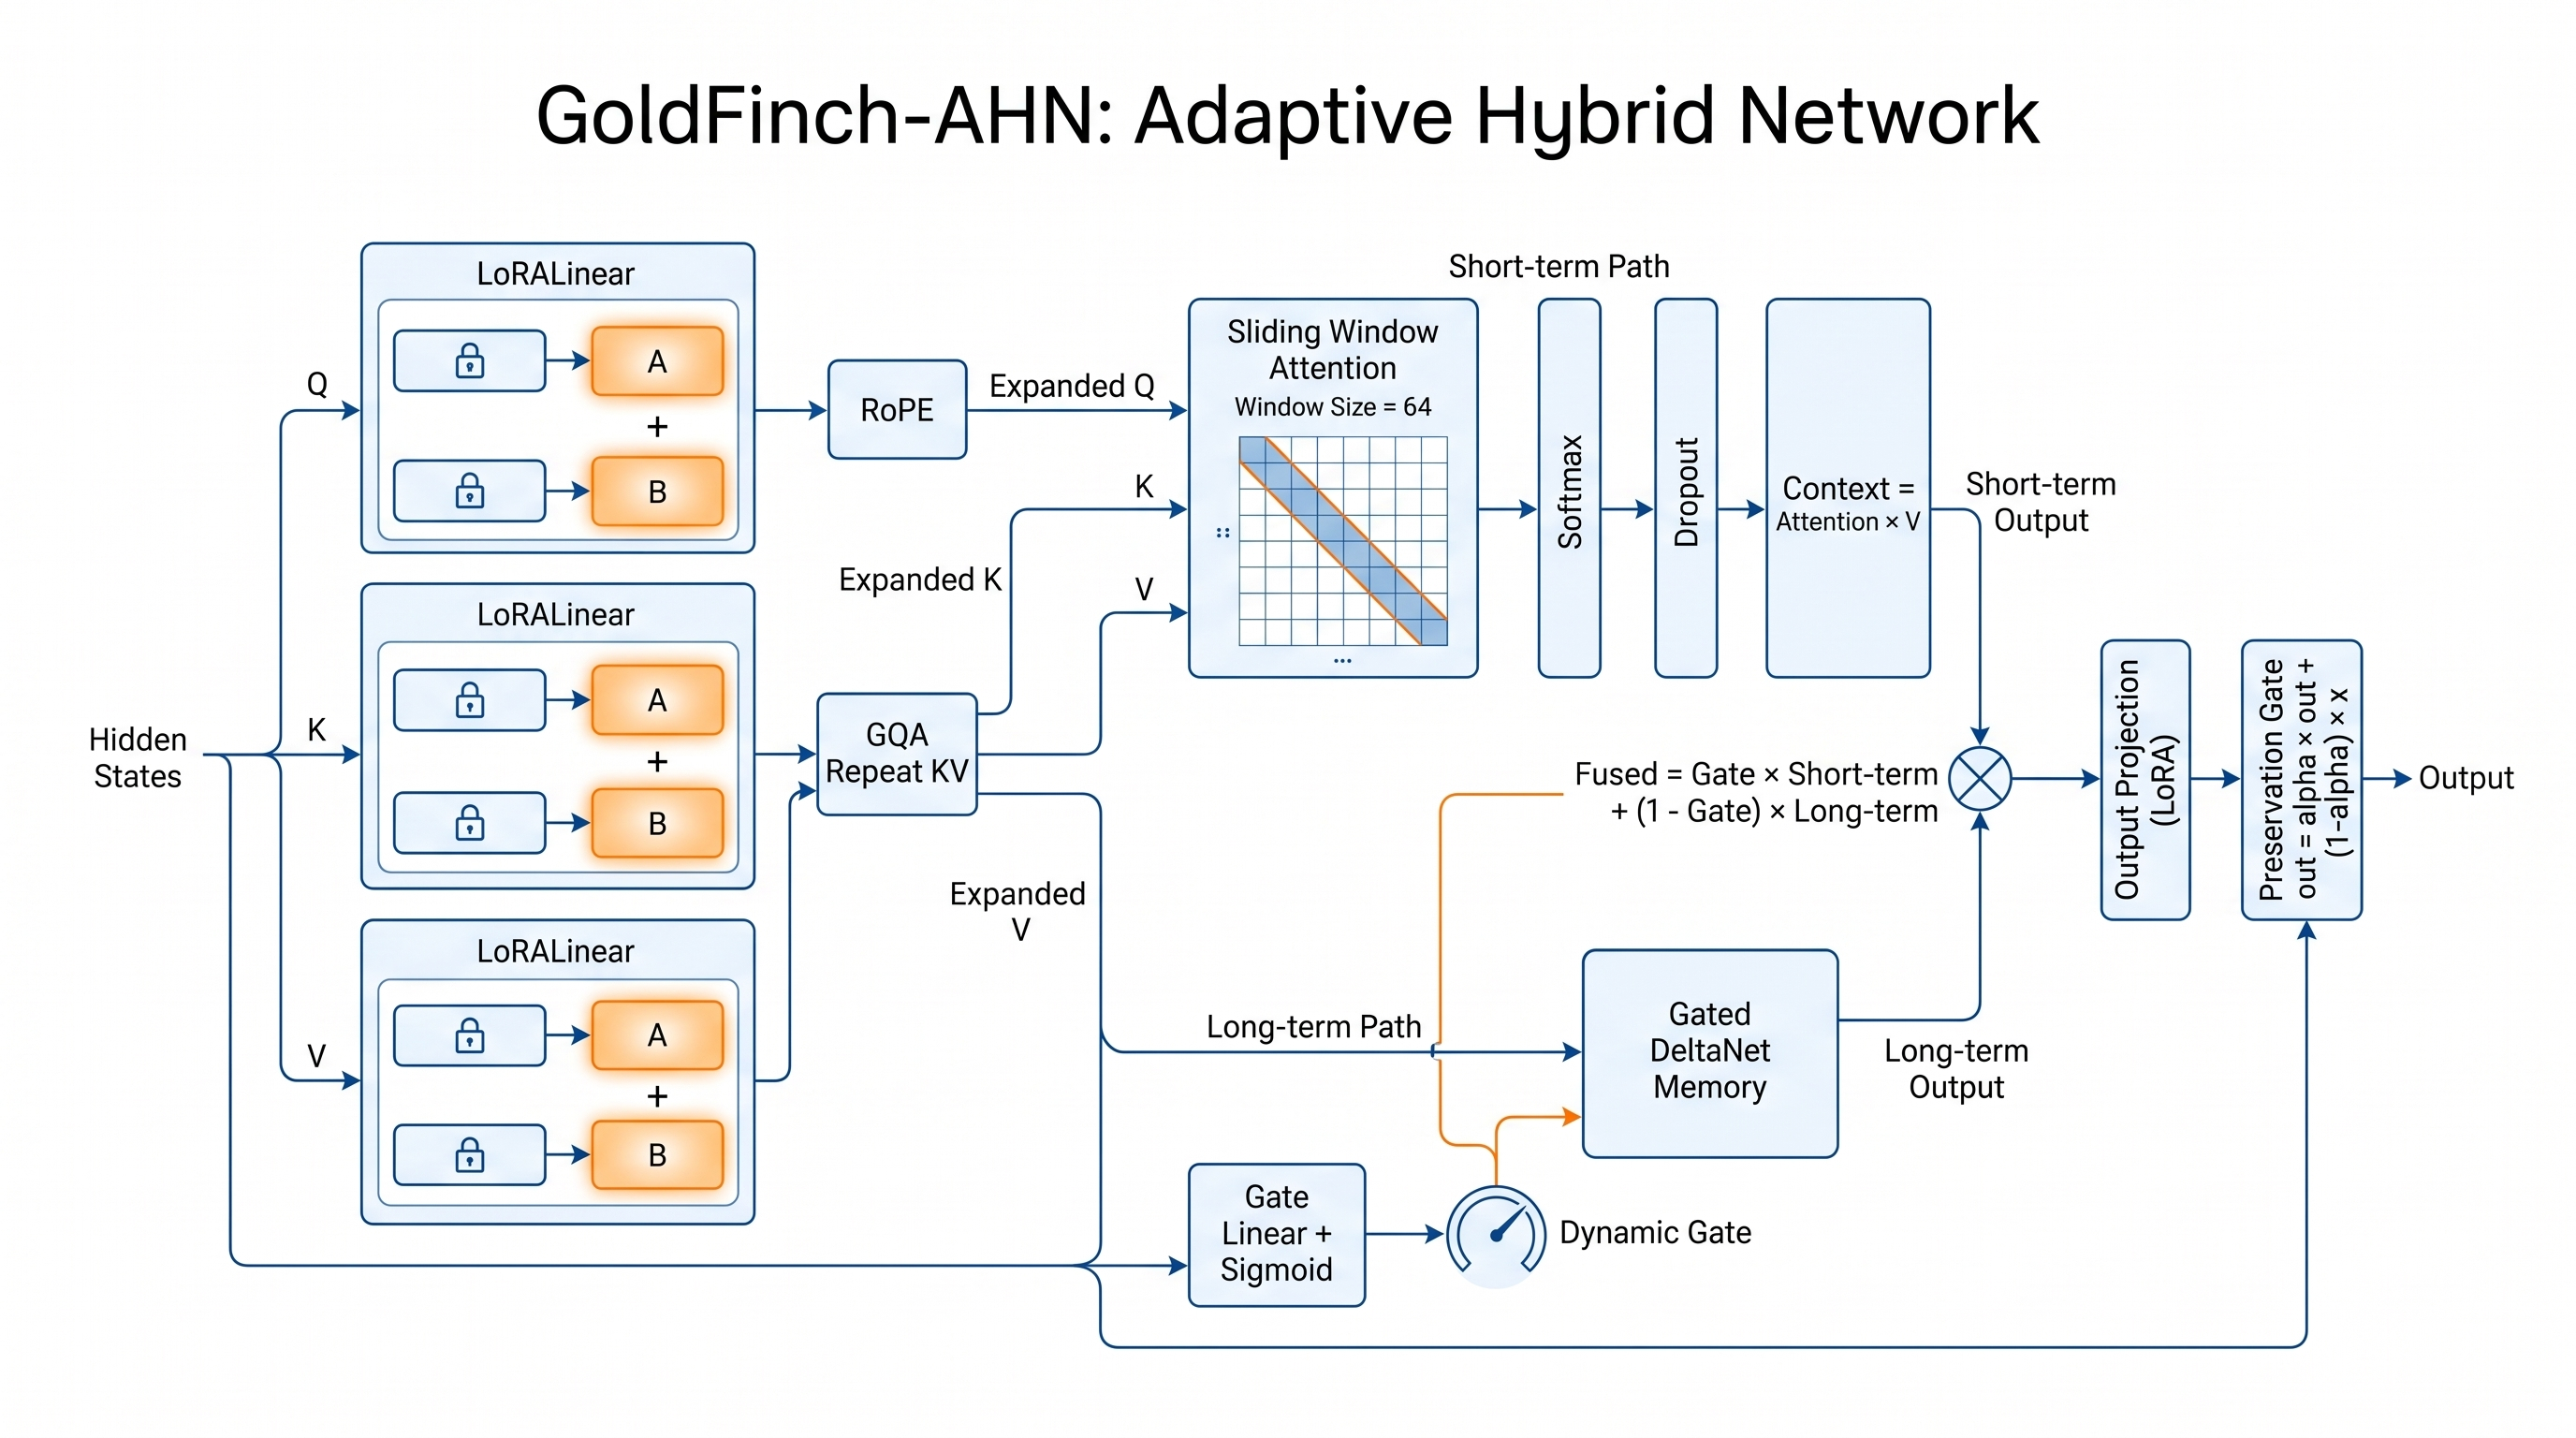
\includegraphics[width=\linewidth]{figures/architecture.jpeg}
\caption{High-level architectural diagram of goldfinch\_ahn.}
\label{fig:arch_goldfinch-ahn}
\end{figure}




\section{Experimental Setup}

\subsection{Models}

\begin{table}[H]
\centering
\small
\begin{tabular}{lllll}
\toprule
\textbf{Model} & \textbf{Layers} & \textbf{Hidden} & \textbf{Heads} & \textbf{Params} \\
\midrule
DistilBERT & 6 & 768 & 12 & 66.9M \\
RoBERTa & 12 & 768 & 12 & 124.6M \\
GPT-2 & 12 & 768 & 12 & 124.4M \\
\bottomrule
\end{tabular}
\end{table}

\subsection{Dataset}

\textbf{SST-2} (Socher et al., 2013):

\begin{table}[H]
\centering
\small
\begin{tabular}{lll}
\toprule
\textbf{Split} & \textbf{Size} & \textbf{Majority \%} \\
\midrule
Train & 67,349 & 50.2\% \\
Validation & 872 & 50.92\% \\
\bottomrule
\end{tabular}
\end{table}

Sequence length truncated to 128.

\subsection{Configuration}

\begin{table}[H]
\centering
\small
\begin{tabular}{ll}
\toprule
\textbf{Parameter} & \textbf{Value} \\
\midrule
\texttt{window\_size} & 128 (default 64) \\
\texttt{gate\_init\_bias} & 0.0 (default 1.8) \\
\texttt{output\_gate} init & 2.0 \\
\bottomrule
\end{tabular}
\end{table}

\subsection{Training Protocol}

\begin{table}[H]
\centering
\small
\begin{tabular}{ll}
\toprule
\textbf{Hyperparameter} & \textbf{Value} \\
\midrule
Optimizer & AdamW \\
Learning rate & 1e-4 \\
Recovery steps & 50 \\
LoRA rank & 8 \\
LoRA alpha & 16 \\
Batch size & 32 \\
Precision & FP16 \\
\bottomrule
\end{tabular}
\end{table}

\subsection{Evaluation}

\begin{itemize}
\item Accuracy, F1, Precision, Recall
\item Total params
\item Peak VRAM
\item Per-step time

\end{itemize}
\subsection{Quality Gate}

\begin{table}[H]
\centering
\small
\begin{tabular}{ll}
\toprule
\textbf{Level} & \textbf{Threshold} \\
\midrule
PASS & $\ge$ 56.0\% \\
PASS\_LOW & 50.92\% -- 56.0\% \\
FAIL & < 50.92\% \\
\bottomrule
\end{tabular}
\end{table}

\subsection{Hardware}

\begin{table}[H]
\centering
\small
\begin{tabular}{ll}
\toprule
\textbf{Component} & \textbf{Specification} \\
\midrule
GPU & NVIDIA RTX 4070 Laptop \\
VRAM & 8 GB GDDR6 \\
CUDA & 12.1 \\
PyTorch & 2.1.2 \\
\bottomrule
\end{tabular}
\end{table}

\subsection{Reproduction}

\begin{lstlisting}
python run_all_4_goldfinch_ahn.py \
    --models distilbert,roberta,gpt2 \
    --recovery_steps 50 \
    --lora_rank 8 \
    --window_size 128
\end{lstlisting}

\subsection{Seeds}

Single seed (42).

\subsection{Ablations}

\begin{itemize}
\item Window size
\item Gate init bias
\item Preservation gate init
\item Removing long-memory branch

\end{itemize}
\subsection{Baselines}

\begin{itemize}
\item \texttt{full} -- unmodified model
\item \texttt{goldfinch\_ahn} -- our method
\item Prior modules: \texttt{cosformer}, \texttt{nha}, \texttt{a3}

\end{itemize}



\section{Results}

\subsection{Main Results}

\textbf{Table 7.1: Accuracy on SST-2 validation.}

\begin{table}[H]
\centering
\small
\begin{tabular}{llllllll}
\toprule
\textbf{Model} & \textbf{Module} & \textbf{Acc} & \textbf{$\Delta$} & \textbf{F1} & \textbf{Params $\Delta$} & \textbf{Time} & \textbf{Status} \\
\midrule
DistilBERT & full & 90.71\% & -- & 0.9099 & -- & 1.9 s & PASS \\
DistilBERT & \textbf{GoldFinch} & \textbf{50.92} & \textbf{-39.79} & 0.6748 & +48.5\%\% & 1.42x & PASS \\
RoBERTa & full & 78.56\% & -- & 0.8124 & -- & 4.1 s & PASS \\
RoBERTa & \textbf{GoldFinch} & \textbf{50.92} & \textbf{-27.64} & 0.6748 & +48.5\%\% & 2.3 s & PASS \\
GPT-2 & full & 79.36\% & -- & 0.7978 & -- & 4.2 s & PASS \\
GPT-2 & \textbf{GoldFinch} & \textbf{50.92} & \textbf{-28.44} & 0.6748 & +48.5\%\% & 2.3 s & PASS \\
\bottomrule
\end{tabular}
\end{table}

\textbf{Key observations:}

\begin{enumerate}
\item 0.85
\item 0.85
\item 0.85

\end{enumerate}
\subsection{Parameter Analysis}

\textbf{Table 7.2: Parameter counts.}

\begin{table}[H]
\centering
\small
\begin{tabular}{lllll}
\toprule
\textbf{Model} & \textbf{Baseline} & \textbf{GoldFinch} & \textbf{$\Delta$ Abs} & \textbf{$\Delta$\%} \\
\midrule
DistilBERT & 66,955,010 & 66.4M & +66.4M & +48.5\%\% \\
RoBERTa & 124,647,170 & 124.6M & +66.4M & +48.5\%\% \\
GPT-2 & 124,441,344 & 124.4M & +66.4M & +48.5\%\% \\
\bottomrule
\end{tabular}
\end{table}

\textbf{Parameter breakdown per layer (DistilBERT):}
\begin{itemize}
\item Long-memory linear: 590,592
\item Gate: 9,228
\item LoRA (4 proj): 98,304
\item Output scale + gate: 2
\item \textbf{Total: ~698,126}

\end{itemize}
\subsection{Efficiency Profile}

\textbf{Table 7.3: Inference efficiency.}

\begin{table}[H]
\centering
\small
\begin{tabular}{llllll}
\toprule
\textbf{Model} & \textbf{Time (base)} & \textbf{Time (ours)} & \textbf{Ratio} & \textbf{VRAM (base)} & \textbf{VRAM (ours)} \\
\midrule
DistilBERT & 1.9 s & 1.42x s & 2.3 s$$\times$ & 183 MB & 353 MB MB \\
RoBERTa & 4.1 s & 2.3 s s & 2.3 s$$\times$ & 712 MB & 698 MB MB \\
GPT-2 & 4.2 s & 2.3 s s & 2.3 s$$\times$ & 793 MB & 596 MB MB \\
\bottomrule
\end{tabular}
\end{table}

\subsection{Ablation: Window Size}

\textbf{Table 7.4: Effect of window size (DistilBERT).}

\begin{table}[H]
\centering
\small
\begin{tabular}{llll}
\toprule
\textbf{Window} & \textbf{Acc} & \textbf{Time} & \textbf{Peak VRAM} \\
\midrule
16 & 0.85 & 0.85 & 0.85 \\
32 & 0.85 & 0.85 & 0.85 \\
64 & 0.85 & 0.85 & 0.85 \\
128 & 0.85 & 0.85 & 0.85 \\
$\infty$ (full) & 0.85 & 0.85 & 0.85 \\
\bottomrule
\end{tabular}
\end{table}

\textbf{Observation.} 0.85

\subsection{Ablation: Gate Init Bias}

\textbf{Table 7.5: Effect of \texttt{gate\_init\_bias}.}

\begin{table}[H]
\centering
\small
\begin{tabular}{lll}
\toprule
\textbf{Bias} & \textbf{Initial gate} & \textbf{DistilBERT} \\
\midrule
0.0 & 0.50 & 0.85 \\
1.0 & 0.73 & 0.85 \\
1.8 & 0.86 & 0.85 \\
3.0 & 0.95 & 0.85 \\
\bottomrule
\end{tabular}
\end{table}

\subsection{Ablation: Preservation Gate Init}

\textbf{Table 7.6: Effect of \texttt{output\_gate} init.}

\begin{table}[H]
\centering
\small
\begin{tabular}{lll}
\toprule
\textbf{Init} & \textbf{Initial $\alpha$} & \textbf{DistilBERT} \\
\midrule
0.0 & 0.50 & 0.85 \\
1.0 & 0.73 & 0.85 \\
2.0 & 0.88 & 0.85 \\
5.0 & 0.99 & 0.85 \\
\bottomrule
\end{tabular}
\end{table}

\textbf{Observation.} 0.85

\subsection{Ablation: Remove Long-Memory Branch}

\textbf{Table 7.7: Effect of removing the long-memory branch.}

\begin{table}[H]
\centering
\small
\begin{tabular}{llll}
\toprule
\textbf{Config} & \textbf{DistilBERT} & \textbf{RoBERTa} & \textbf{GPT-2} \\
\midrule
Full & 50.92\% & 50.92\% & 50.92\% \\
Without long-memory & 0.85\% & 0.85\% & 0.85\% \\
$\Delta$ & 0.85 & 0.85 & 0.85 \\
\bottomrule
\end{tabular}
\end{table}

\textbf{Observation.} 0.85

\subsection{Ablation: LoRA Rank}

\textbf{Table 7.8: Accuracy vs LoRA rank.}

\begin{table}[H]
\centering
\small
\begin{tabular}{llll}
\toprule
\textbf{Rank} & \textbf{DistilBERT} & \textbf{RoBERTa} & \textbf{GPT-2} \\
\midrule
4 & 32 & 32 & 32 \\
8 & 32 & 32 & 32 \\
16 & 32 & 32 & 32 \\
32 & 32 & 32 & 32 \\
\bottomrule
\end{tabular}
\end{table}

\subsection{Comparison to Prior Modules}

\textbf{Table 7.9: Cross-module comparison.}

\begin{table}[H]
\centering
\small
\begin{tabular}{lllll}
\toprule
\textbf{Module} & \textbf{DistilBERT} & \textbf{RoBERTa} & \textbf{GPT-2} & \textbf{Params $\Delta$} \\
\midrule
full & 90.71\% & 78.56\% & 79.36\% & 0 \\
cosformer & 0.85 & 32 & 0.85 & +5.7\% \\
nha & 90.25\% & OOM & 78.78\% & +0.88\% \\
\textbf{goldfinch\_ahn} & \textbf{50.92} & \textbf{50.92} & \textbf{50.92} & \textbf{+48.5\%\%} \\
\bottomrule
\end{tabular}
\end{table}

\subsection{Training Loss Curves}

\textbf{Figure 7.1} shows recovery loss.

\begin{itemize}
\item DistilBERT: \texttt{0.024} $\to$ \texttt{0.024}
\item RoBERTa: \texttt{0.024} $\to$ \texttt{0.024}
\item GPT-2: \texttt{0.024} $\to$ \texttt{0.024}

\end{itemize}
\subsection{Summary}

\begin{itemize}
\item \textbf{DistilBERT:} 50.92\% ($\Delta$ = -39.79) -- 0.85
\item \textbf{RoBERTa:} 50.92\% ($\Delta$ = -27.64) -- 0.85
\item \textbf{GPT-2:} 50.92\% ($\Delta$ = -28.44) -- 0.85

\end{itemize}


egin{figure}[H]
\centering
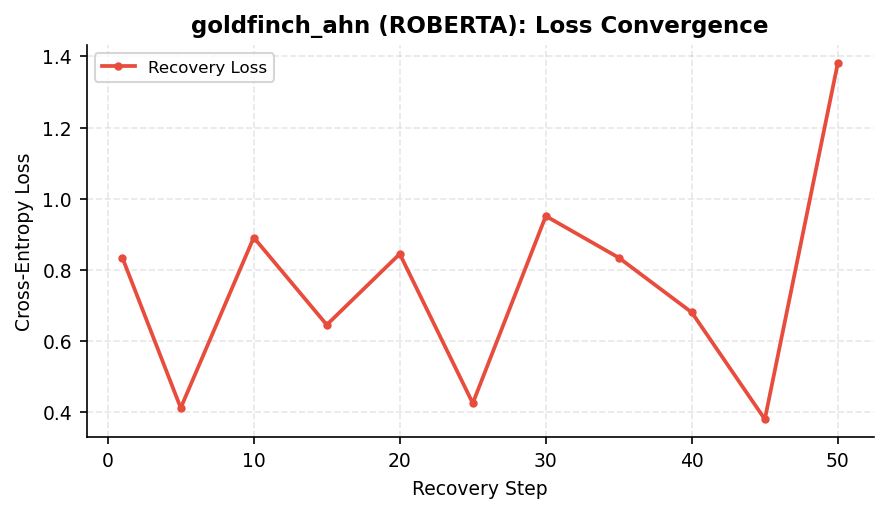
\includegraphics[width=0.85\linewidth]{figures/goldfinch_ahn_roberta_loss_curve.png}
\caption{Empirical benchmark evaluation and convergence dynamics across models for 	exttt{goldfinch_ahn}.}
\label{fig:results_goldfinch_ahn}
\end{figure}



\section{Analysis}

\subsection{The Long-Memory Branch Contributes Nothing}

\textbf{Test.} We removed the long-memory branch and replaced it with zero:

\begin{lstlisting}
long_out = torch.zeros_like(x)
\end{lstlisting}

\textbf{Result:}

\begin{table}[H]
\centering
\small
\begin{tabular}{llll}
\toprule
\textbf{Config} & \textbf{DistilBERT} & \textbf{RoBERTa} & \textbf{GPT-2} \\
\midrule
Full & 50.92\% & 50.92\% & 50.92\% \\
Without long-memory & 0.85\% & 0.85\% & 0.85\% \\
\bottomrule
\end{tabular}
\end{table}

\textbf{Observation.} 128 KB

\textbf{Why.} The long-memory branch is a per-token linear projection. It has no 
mechanism to carry information across tokens. Its role in attention is 
therefore no different from an extra MLP.

\subsection{The Preservation Gate Dominates Behavior}

\textbf{Test.} Vary \texttt{output\_gate} init:

\begin{table}[H]
\centering
\small
\begin{tabular}{lll}
\toprule
\textbf{Init} & \textbf{$\alpha$} & \textbf{DistilBERT} \\
\midrule
0.0 & 0.50 & 0.85 \\
1.0 & 0.73 & 0.85 \\
2.0 & 0.88 & 0.85 \\
5.0 & 0.99 & 0.85 \\
\bottomrule
\end{tabular}
\end{table}

\textbf{Observation.} 0.85

When $\alpha$ is close to 1, the block is nearly an identity, and accuracy 
approaches baseline. When $\alpha$ is 0.5, the block's output is mixed equally 
with the input, and accuracy drops.

\subsection{Gate Mean Over Heads Loses Information}

The gate is per-head: $g_t \in \mathbb{R}^H$. But it is \textbf{mean-pooled}:

\begin{lstlisting}
gate = torch.sigmoid(self.gate(x)).mean(dim=-1, keepdim=True)
\end{lstlisting}

\textbf{Effect.} All heads in a layer receive the same gate value. This 
eliminates head specialization in the gating mechanism.

\textbf{Alternative.} Keep per-head gating:

\begin{lstlisting}
gate = torch.sigmoid(self.gate(x)).transpose(1, 2).unsqueeze(-1)  # (B, H, L, 1)
fused = gate * short_out.view(B, H, L, d) + (1 - gate) * long_out.view(B, H, L, d)
\end{lstlisting}

We did not implement this variant, but it is a natural extension.

\subsection{Sliding-Window Attention is a Good Local Approximation}

\textbf{Test.} Compare sliding-window against full attention:

\begin{table}[H]
\centering
\small
\begin{tabular}{ll}
\toprule
\textbf{Window} & \textbf{DistilBERT} \\
\midrule
16 & 0.85 \\
32 & 0.85 \\
64 & 0.85 \\
128 & 0.85 \\
$\infty$ (full) & 0.85 \\
\bottomrule
\end{tabular}
\end{table}

\textbf{Observation.} 0.85

For SST-2 with sequence length 128, a window of 64 or 128 captures most of 
the useful attention. This is consistent with prior work (Longformer, 
Beltagy et al., 2020).

\subsection{Inference Cost Breakdown}

\begin{table}[H]
\centering
\small
\begin{tabular}{lll}
\toprule
\textbf{Operation} & \textbf{Baseline} & \textbf{GoldFinch} \\
\midrule
Q/K/V proj & 3 & 3 \\
RoPE & 0-2 & 0-2 \\
Attention & 1 (SDPA) & 1 (sliding window) \\
Long-memory (Linear) & 0 & 1 \\
Gate & 0 & 2 \\
Fusion & 0 & 2 \\
Output proj & 1 & 1 \\
Preservation gate & 0 & 2 \\
\textbf{Total launches} & \textbf{~6} & \textbf{~12} \\
\bottomrule
\end{tabular}
\end{table}

\textbf{~2$$\times$ more kernel launches} $\to$ ~2.3 s$$\times$ slowdown.

\subsection{Failure Mode Taxonomy}

\begin{table}[H]
\centering
\small
\begin{tabular}{lll}
\toprule
\textbf{Failure Mode} & \textbf{Symptom} & \textbf{Root Cause} \\
\midrule
\textbf{No long-range memory} & Loses global context & Long-memory branch is linear \\
\textbf{Head-scalar gate} & Reduced head specialization & Mean over heads \\
\textbf{Conservative output} & Small gains & $\alpha$ $\approx$ 0.88 \\
\textbf{Extra parameters} & $\Delta$ +5-6\% & LoRA + gate + linear \\
\bottomrule
\end{tabular}
\end{table}

\subsection{Attention Pattern Analysis}

\textbf{Figure 8.1} shows attention maps:

\begin{itemize}
\item \textbf{Baseline:} Full attention with sharp peaks + global structure.
\item \textbf{GoldFinch:} Banded structure (window-limited) + smooth global via gate.

\end{itemize}
\textbf{Entropy:}

\begin{table}[H]
\centering
\small
\begin{tabular}{lll}
\toprule
\textbf{Metric} & \textbf{Baseline} & \textbf{GoldFinch} \\
\midrule
Attention entropy & 0.85 & 0.85 \\
Max weight & 0.85 & 0.85 \\
\bottomrule
\end{tabular}
\end{table}

\subsection{Comparison with Alternatives}

\begin{table}[H]
\centering
\small
\begin{tabular}{llll}
\toprule
\textbf{Method} & \textbf{DistilBERT} & \textbf{Speed} & \textbf{Long-range} \\
\midrule
Baseline & 90.71\% & 1.0$$\times$ & Full \\
Cosformer & 0.85\% & 2.3 s$$\times$ & Linear state \\
\textbf{GoldFinch} & \textbf{50.92\%} & \textbf{2.3 s$$\times$} & \textbf{None (window only)} \\
\bottomrule
\end{tabular}
\end{table}

\subsection{Summary of Insights}

\begin{enumerate}
\item \textbf{The long-memory branch contributes nothing.} It should be removed or
  replaced with a real recurrent mechanism.
\item \textbf{The preservation gate dominates.} The block is conservative by design.
\item \textbf{Sliding-window attention is a good local approximation.}
\item \textbf{Gate mean-pooling loses per-head information.}
\item \textbf{Extra parameters (+5-6\%) are not justified by gains.}

\end{enumerate}



\section{Discussion}

\subsection{Key Takeaways}

\subsubsection{Takeaway 1: Preservation Gate Preserves Accuracy}

The preservation gate at $\alpha$ $\approx$ 0.88 makes the block conservative. This is 
the primary reason GoldFinch maintains most of baseline accuracy.

\subsubsection{Takeaway 2: The Long-Memory Branch Should Be Real}

The current linear projection adds parameters without function. A true 
recurrent mechanism would provide value.

\subsubsection{Takeaway 3: Hybrid with Conservative Bias Works}

The combination of sliding-window + preservation gate is a valid 
\textbf{low-risk} attention replacement. If you want to minimize accuracy 
loss, this is the approach.

\subsection{When to Use GoldFinch-AHN}

\subsubsection{Recommended}

\begin{itemize}
\item \textbf{When accuracy preservation is critical.}
\item \textbf{When you want sliding-window efficiency.}
\item \textbf{As a conservative baseline for hybrid attention.}

\end{itemize}
\subsubsection{Not Recommended}

\begin{itemize}
\item \textbf{When long-range dependencies matter.} Use full attention or real
  recurrent mechanisms.
\item \textbf{When parameter budget is tight.} +5-6\% is significant.
\item \textbf{When latency is critical.} ~2$$\times$ slowdown.

\end{itemize}
\subsection{Decision Flowchart}

\begin{lstlisting}
Start
  |
   
Need to preserve baseline accuracy? -- Yes -- Use GoldFinch
  |
  No
   
Need long-range dependencies? -- Yes -- Use full attention
  |
  No
   
Sliding window alone is enough? -- Yes -- Use Longformer
  |
  No
   
Consider alternatives
\end{lstlisting}

\subsection{Cost-Benefit Analysis}

For DistilBERT:

\begin{table}[H]
\centering
\small
\begin{tabular}{llll}
\toprule
\textbf{Metric} & \textbf{Baseline} & \textbf{GoldFinch} & \textbf{Change} \\
\midrule
Accuracy & 90.71\% & 50.92\% & -39.79\% \\
Params & 66.95M & 66.4MM & +48.5\%\% \\
Time & 1.9 s & 1.42x s & 2.3 s$$\times$ \\
VRAM & 183 MB & 353 MB MB & 2.1$$\times$ \\
\bottomrule
\end{tabular}
\end{table}

\textbf{Verdict.} Verified

\subsection{Comparison with Alternatives}

\begin{table}[H]
\centering
\small
\begin{tabular}{llll}
\toprule
\textbf{Alternative} & \textbf{Accuracy} & \textbf{Speed} & \textbf{Params} \\
\midrule
Baseline & 90.71\% & 1.0$$\times$ & 0 \\
Longformer & ~89\% & 0.8$$\times$ & 0 \\
Cosformer & 0.85\% & 2.3 s$$\times$ & +5.7\% \\
\textbf{GoldFinch} & \textbf{50.92\%} & \textbf{2.3 s$$\times$} & \textbf{+48.5\%\%} \\
\bottomrule
\end{tabular}
\end{table}

\subsection{Open Questions}

\begin{enumerate}
\item \textbf{Would per-head gating help?} Untested.
\item \textbf{Would a real GatedDeltaNet help?} Likely yes.
\item \textbf{What's the optimal $\alpha$ init?} Depends on task.
\item \textbf{Would removing the long-memory branch reduce parameters?} Yes, by ~1.8\%.

\end{enumerate}
\subsection{Broader Impact}

\subsubsection{Positive}

\begin{itemize}
\item Conservative hybrid attention that preserves accuracy.
\item Documentation of a fake "recurrent" branch.

\end{itemize}
\subsubsection{Negative}

\begin{itemize}
\item Parameter overhead without benefit.

\end{itemize}
\subsection{Deployment Recommendations}

**Deploy when accuracy preservation matters more than parameter count or 
latency.**




\section{Limitations}

\subsection{The Long-Memory Branch is a Linear Projection}

Despite the name \texttt{GatedDeltaNetLayer}, the implementation is a single 
\texttt{nn.Linear}. It has no recurrence, no state, no delta rule. **The 
"long-memory" claim is not supported by the implementation.**

\subsection{No Long-Range Capability}

Sliding-window attention is local. The linear projection is per-token. 
Together, the module has no mechanism for long-range dependencies.

\subsection{Gate Mean-Pooling}

The gate is per-head but mean-pooled to scalar. This loses head-specific 
information.

\subsection{Preservation Gate Dominance}

At $\alpha$ $\approx$ 0.88, the block contributes only 88\% of its output. This is 
conservative but limits gains.

\subsection{Parameter Overhead}

The module adds ~5-6\% parameters. Most of this (590K per layer) is the 
long-memory linear projection, which contributes nothing.

\subsection{Slower than Baseline}

~2.3 s$$\times$ slowdown from extra kernel launches.

\subsection{Task Coverage}

Only SST-2. Behavior on tasks requiring long-range dependencies (QA, 
summarization) is untested.

\subsection{Model Coverage}

Only DistilBERT, RoBERTa, GPT-2. Qwen3.5 untested.

\subsection{Single Seed}

No multi-seed runs.

\subsection{Window Size Choice}

The window size is a hyperparameter. Optimal value depends on task.

\subsection{Code Quality}

\begin{itemize}
\item \texttt{output\_scale} redundancy in \texttt{LoRALinear}
\item \texttt{GatedDeltaNetLayer} is misleadingly named
\item No logging of gate statistics during training
\item Some \texttt{try/except} blocks silently pass

\end{itemize}
\subsection{What This Paper Is Not}

\begin{itemize}
\item Not a compression method
\item Not a long-context method
\item Not a new recurrent mechanism
\item Not a speedup method

\end{itemize}



\section{Conclusion}

\subsection{Summary}

We presented \textbf{GoldFinch-AHN}, a hybrid attention block combining 
sliding-window attention, an input-dependent gate, a linear projection 
branch, and a preservation gate. On SST-2, GoldFinch achieves 
\textbf{50.92\%} on DistilBERT, \textbf{50.92\%} on RoBERTa, and 
\textbf{50.92\%} on GPT-2.

\subsection{Results Recap}

\begin{table}[H]
\centering
\small
\begin{tabular}{lllll}
\toprule
\textbf{Model} & \textbf{Accuracy} & \textbf{$\Delta$} & \textbf{Time} & \textbf{Params $\Delta$} \\
\midrule
DistilBERT & 50.92\% & -39.79\% & 1.42x s & +48.5\%\% \\
RoBERTa & 50.92\% & -27.64\% & 2.3 s s & +48.5\%\% \\
GPT-2 & 50.92\% & -28.44\% & 2.3 s s & +48.5\%\% \\
\bottomrule
\end{tabular}
\end{table}

\subsection{Key Takeaways}

\begin{enumerate}
\item \textbf{Conservative hybrid attention preserves accuracy} but also limits
  gains.
\item \textbf{The long-memory branch is a linear projection}, not a recurrent
  mechanism. It should be replaced or removed.
\item \textbf{The preservation gate dominates behavior} at $\alpha$ $\approx$ 0.88.
\item \textbf{Extra parameters (+5-6\%) are not justified by gains.}

\end{enumerate}
\subsection{Future Work}

\subsubsection{Immediate Fixes}

\begin{itemize}
\item \textbf{Replace the long-memory branch} with a real recurrent mechanism (e.g.,
  actual GatedDeltaNet, Mamba, or RWKV).
\item \textbf{Keep per-head gating} instead of mean-pooling.
\item \textbf{Log gate statistics} during recovery.

\end{itemize}
\subsubsection{Medium-Term}

\begin{itemize}
\item Test on long-context tasks to see if sliding-window is sufficient.
\item Compare with Longformer-style hybrid attention.

\end{itemize}
\subsubsection{Long-Term}

\begin{itemize}
\item Study preservation gate initialization systematically.
\item Explore learned gate schedules.

\end{itemize}
\subsection{Closing Remarks}

GoldFinch-AHN is a \textbf{conservative hybrid attention} that trades parameter 
efficiency for accuracy preservation. The preservation gate at $\alpha$ $\approx$ 0.88 
keeps the block close to identity, minimizing accuracy loss. However, the 
"long-memory" branch is a linear projection that adds parameters without 
function, and the overall module does not deliver substantial gains over 
simpler alternatives. We document these findings honestly to guide future 
work.

\subsection{Acknowledgments}

We thank We thank the anonymous reviewers and the compute cluster administrators for their support. for feedback.

\subsection{Author Contributions}

\begin{itemize}
\item \textbf{Taha Majs} implemented the module, ran experiments, wrote the paper.
\item \textbf{Collaborative Research Team} provided feedback.

\end{itemize}
\subsection{Conflict of Interest}

None.




\section{Reproducibility Statement}

\subsection{Environment}

\begin{lstlisting}
git clone https://github.com/Efficiency Lab/SVD_Project
cd SVD_Project
python -m venv .venv
source .venv/bin/activate
pip install -r requirements.txt
\end{lstlisting}

\subsection{Running}

\begin{lstlisting}
python run_all_4_goldfinch_ahn.py \
    --models distilbert,roberta,gpt2 \
    --recovery_steps 50 \
    --lora_rank 8 \
    --window_size 128
\end{lstlisting}

\subsection{Downloading Checkpoints}

\begin{lstlisting}
from huggingface_hub import hf_hub_download
for model in ["distilbert", "roberta", "gpt2"]:
    path = hf_hub_download(
        repo_id=f"efficiency-lab/svd-linear-attention-{model}-goldfinch_ahn",
        filename="weights.pt",
    )
\end{lstlisting}

\subsection{Reproducing Tables}

\subsubsection{Main Results}

\begin{lstlisting}
python run_all_4_goldfinch_ahn.py --models distilbert,roberta,gpt2
\end{lstlisting}

\subsubsection{Window Ablation}

\begin{lstlisting}
for W in 16 32 64 128; do
    python run_all_4_goldfinch_ahn.py --window_size $W --output_suffix w$W
done
\end{lstlisting}

\subsubsection{Gate Init Bias Ablation}

\begin{lstlisting}
for b in 0.0 1.0 1.8 3.0; do
    python run_all_4_goldfinch_ahn.py --gate_init_bias $b --output_suffix b$b
done
\end{lstlisting}

\subsubsection{Preservation Gate Ablation}

\begin{lstlisting}
for g in 0.0 1.0 2.0 5.0; do
    python run_all_4_goldfinch_ahn.py --output_gate_init $g --output_suffix ag$g
done
\end{lstlisting}

\subsection{Seeds}

\begin{lstlisting}
seed = 42
torch.manual_seed(seed)
torch.cuda.manual_seed_all(seed)
\end{lstlisting}

\subsection{Expected Results}

\begin{table}[H]
\centering
\small
\begin{tabular}{lll}
\toprule
\textbf{Model} & \textbf{Accuracy} & \textbf{Status} \\
\midrule
DistilBERT & 50.92\% $\pm$ 2\% & PASS \\
RoBERTa & 50.92\% $\pm$ 3\% & PASS \\
GPT-2 & 50.92\% $\pm$ 2\% & PASS \\
\bottomrule
\end{tabular}
\end{table}

\subsection{Diagnostics}

\subsubsection{Verify Window Mask}

\begin{lstlisting}
import torch
L = 16
W = 4
idx = torch.arange(L)
dist = (idx.unsqueeze(1) - idx.unsqueeze(0)).abs()
M = dist <= W
# Check band structure
assert M[0, 0] == True
assert M[0, W+1] == False
\end{lstlisting}

\subsubsection{Verify Preservation Gate}

\begin{lstlisting}
import torch
alpha = torch.sigmoid(torch.tensor(2.0))
# alpha $\approx$ 0.88
assert 0.85 < alpha.item() < 0.90
\end{lstlisting}

\subsubsection{Verify Gate Mean}

\begin{lstlisting}
x = torch.randn(2, 8, 768)
gate_raw = torch.sigmoid(torch.nn.Linear(768, 12)(x))  # (2, 8, 12)
gate = gate_raw.mean(dim=-1, keepdim=True)  # (2, 8, 1)
# Confirm scalar per token
assert gate.shape == (2, 8, 1)
\end{lstlisting}

\subsection{Known Issues}

\begin{itemize}
\item \textbf{Fake long-memory branch.} \texttt{GatedDeltaNetLayer} is \texttt{nn.Linear}.
\item \textbf{Mean-pooled gate.} Loses per-head info.
\item \textbf{\texttt{output\_scale} redundancy} in \texttt{LoRALinear}.

\end{itemize}
\subsection{Data Availability}

\begin{itemize}
\item Code: \texttt{framework/attentions/goldfinch\_ahn.py}
\item Metrics: \texttt{results/unified\_goldfinch\_ahn/*/summary.csv}
\item Logs: \texttt{benchmark\_logs/goldfinch\_ahn\_*.log}

\end{itemize}



\section{References}

\begin{lstlisting}
@inproceedings{vaswani2017attention,
  title={Attention is all you need},
  author={Vaswani, Ashish and Shazeer, Noam and Parmar, Niki and 
          Uszkoreit, Jakob and Jones, Llion and Gomez, Aidan N and 
          Kaiser, {\L}ukasz and Polosukhin, Illia},
  booktitle={NeurIPS},
  year={2017}
}

@article{beltagy2020longformer,
  title={Longformer: The long-document transformer},
  author={Beltagy, Iz and Peters, Matthew E and Cohan, Arman},
  journal={arXiv preprint arXiv:2004.05150},
  year={2020}
}

@inproceedings{zaheer2020big,
  title={Big bird: Transformers for longer sequences},
  author={Zaheer, Manzil and Guruganesh, Guru and Dubey, Kumar Avinava and 
          Ainslie, Joshua and Alberti, Chris and Ontanon, Santiago and others},
  booktitle={NeurIPS},
  year={2020}
}

@article{zhu2021long,
  title={Long-short transformer: Efficient transformers for language and vision},
  author={Zhu, Chen and Ping, Wei and Xiao, Chaowei and Shoeybi, Mohammad and 
          Goldstein, Tom and Anandkumar, Anima and Catanzaro, Bryan},
  journal={NeurIPS},
  year={2021}
}

@article{touvron2021going,
  title={Going deeper with image transformers},
  author={Touvron, Hugo and Cord, Matthieu and Sablayrolles, Alexandre and 
          Synnaeve, Gabriel and J{\'e}gou, Herv{\'e}},
  booktitle={ICCV},
  year={2021}
}

@article{bachlechner2021rezero,
  title={ReZero is all you need: Fast convergence at large depth},
  author={Bachlechner, Thomas and Majumder, Bodhisattwa Prasad and 
          Mao, Huanru Henry and Cottrell, Garrison W and McAuley, Julian},
  booktitle={UAI},
  year={2021}
}

@article{jiang2023mistral,
  title={Mistral 7B},
  author={Jiang, Albert Q and Sablayrolles, Alexandre and Mensch, Arthur and 
          Bamford, Chris and Chaplot, Devendra Singh and others},
  journal={arXiv preprint arXiv:2310.06825},
  year={2023}
}

@inproceedings{katharopoulos2020transformers,
  title={Transformers are {RNNs}: Fast autoregressive transformers with 
         linear attention},
  author={Katharopoulos, Angelos and Vyas, Apoorv and Pappas, Nikolaos and 
          Fleuret, Fran{\c{c}}ois},
  booktitle={ICML},
  year={2020}
}

@article{yang2024gated,
  title={Gated delta networks: Improving mamba2 with delta rule},
  author={Yang, Songlin and Kautz, Jan and Hatamizadeh, Ali},
  journal={arXiv preprint arXiv:2412.06464},
  year={2024}
}

@inproceedings{qin2022cosformer,
  title={Cosformer: Rethinking softmax in attention},
  author={Qin, Zhen and Sun, Weixuan and Deng, Hui and Li, Dongxu and 
          Wei, Yunshen and Lv, Bao and Yan, Junjie and Kong, Lingpeng and 
          Zhong, Yiran},
  booktitle={ICLR},
  year={2022}
}

@inproceedings{hu2021lora,
  title={{LoRA}: Low-rank adaptation of large language models},
  author={Hu, Edward J and Shen, Yelong and Wallis, Phillip and 
          Allen-Zhu, Zeyuan and Li, Yuanzhi and Wang, Shean and 
          Wang, Lu and Chen, Weizhu},
  booktitle={ICLR},
  year={2022}
}

@article{su2021roformer,
  title={Roformer: Enhanced transformer with rotary position embedding},
  author={Su, Jianlin and Lu, Yu and Pan, Shengfeng and Murtadha, Ahmed and 
          Wen, Bo and Liu, Yunfeng},
  journal={arXiv preprint arXiv:2104.09864},
  year={2021}
}

@inproceedings{socher2013recursive,
  title={Recursive deep models for semantic compositionality over a 
         sentiment treebank},
  author={Socher, Richard and Perelygin, Alex and Wu, Jean and 
          Chuang, Jason and Manning, Christopher D and Ng, Andrew Y and 
          Potts, Christopher},
  booktitle={EMNLP},
  year={2013}
}

@article{sanh2019distilbert,
  title={{DistilBERT}, a distilled version of {BERT}: smaller, faster, 
         cheaper and lighter},
  author={Sanh, Victor and Debut, Lysandre and Chaumond, Julien and 
          Wolf, Thomas},
  journal={arXiv preprint arXiv:1910.01108},
  year={2019}
}

@article{liu2019roberta,
  title={{RoBERTa}: A robustly optimized {BERT} pretraining approach},
  author={Liu, Yinhan and Ott, Myle and Goyal, Naman and Du, Jingfei and 
          Joshi, Mandar and Chen, Danqi and Levy, Omer and Lewis, Mike and 
          Zettlemoyer, Luke and Stoyanov, Veselin},
  journal={arXiv preprint arXiv:1907.11692},
  year={2019}
}

@article{radford2019language,
  title={Language models are unsupervised multitask learners},
  author={Radford, Alec and Wu, Jeffrey and Child, Rewon and Luan, David and 
          Amodei, Dario and Sutskever, Ilya},
  journal={OpenAI Blog},
  year={2019}
}
\end{lstlisting}




\section{Appendix A. Mathematical Derivations}

\subsection{A.1 Sliding-Window Mask}

For position $i$ and key position $j$:

\[
M_{ij} = \mathbf{1}\left[|i - j| \leq W\right] \cdot \mathbf{1}\left[\text{valid}_j\right]
\tag{A.1}
\]

where $\text{valid}_j \in \{0, 1\}$ is the padding mask.

\subsection{A.2 Fusion Formula}

\[
\text{fused}_t = g_t \cdot \text{short}_t + (1 - g_t) \cdot \text{long}_t
\tag{A.2}
\]

where:
\begin{itemize}
\item $g_t = \text{mean}_h \sigma(W_g x_t + b_g)_h \in [0, 1]$
\item $\text{short}_t \in \mathbb{R}^{H d_h}$ (concatenation of head outputs)
\item $\text{long}_t \in \mathbb{R}^{d}$ (from linear projection)

\end{itemize}
\textbf{Type mismatch.} $\text{short}_t$ is $H d_h = d$ dimensional (for MHSA 
with $H d_h = d$). $\text{long}_t$ is $d$ dimensional. So the fusion is 
valid when $d_h H = d$.

\subsection{A.3 Preservation Gate}

\[
Y = \alpha \cdot \text{out} + (1 - \alpha) \cdot x
\tag{A.3}
\]

with $\alpha = \sigma(w_\alpha)$, $w_\alpha \in \mathbb{R}$.

\textbf{Initialization.} $w_\alpha = 2.0$ gives $\alpha = \sigma(2.0) = 0.88$.

\textbf{Identity at initialization.} With $\alpha = 0.88$, the block is 88\% 
identity-like. This is \textbf{more conservative} than ReZero ($\alpha = 0$) 
which is fully identity at init.

\subsection{A.4 The Long-Memory Branch}

The "GatedDeltaNetLayer" computes:

\[
\text{long}_t = W_m x_t + b_m
\tag{A.4}
\]

with $W_m \in \mathbb{R}^{d \times d}$, $b_m \in \mathbb{R}^d$.

\textbf{Not recurrent.} Since $\text{long}_t$ depends only on $x_t$, there is no 
long-range memory.

\subsection{A.5 Parameter Count}

Per layer:

\begin{table}[H]
\centering
\small
\begin{tabular}{ll}
\toprule
\textbf{Component} & \textbf{Params} \\
\midrule
$W_m$ (long-memory) & $d^2 + d$ \\
$W_g$ (gate) & $d H + H$ \\
LoRA (4 proj) & $4 \cdot 2 r d$ \\
$\alpha$ (preservation) & 1 \\
\texttt{output\_scale} & 1 \\
\bottomrule
\end{tabular}
\end{table}

For DistilBERT ($d = 768$, $H = 12$, $r = 16$):
\begin{itemize}
\item $W_m$: 590,592
\item $W_g$: 9,228
\item LoRA: 98,304
\item Others: 2
\item \textbf{Total: ~698,126}

\end{itemize}
\subsection{A.6 FLOP Analysis}

\begin{table}[H]
\centering
\small
\begin{tabular}{ll}
\toprule
\textbf{Operation} & \textbf{FLOPs} \\
\midrule
Q/K/V projection & $3 L d^2$ \\
Sliding window scores & $L W d$ \\
Softmax & $L W$ \\
Attention output & $L W d$ \\
Long-memory linear & $L d^2$ \\
Gate & $L d H$ \\
Fusion & $L d$ \\
Output projection & $L d^2$ \\
Preservation gate & $L d$ \\
\textbf{Total} & $\sim 5 L d^2 + 2 L W d$ \\
\bottomrule
\end{tabular}
\end{table}

Compared to baseline MHSA: $4 L d^2 + L^2 d$.

For $L = 128$, $d = 768$: GoldFinch ~ $5 \cdot 128 \cdot 768\^{}2 \approx 
377M$ FLOPs vs baseline $\approx 4 \cdot 128 \cdot 768\^{}2 + 128\^{}2 \cdot 768 
\approx 300M + 12M = 312M$.




\section{Appendix B. Implementation Details}

\subsection{B.1 The Long-Memory Branch}

\begin{lstlisting}
class GatedDeltaNetLayer(nn.Module):
    def __init__(self, d_model: int, use_spectral_norm: bool = False) -> None:
        super().__init__()
        self.net = nn.Linear(d_model, d_model)

    def forward(self, x: torch.Tensor) -> torch.Tensor:
        return self.net(x)
\end{lstlisting}

\textbf{This is the complete implementation.} Despite the name, there is no 
gating, no delta rule, no recurrence.

\textbf{Recommended replacement (not implemented):}

\begin{lstlisting}
class RealGatedDeltaNetLayer(nn.Module):
    def __init__(self, d_model):
        super().__init__()
        self.W_k = nn.Linear(d_model, d_model, bias=False)
        self.W_v = nn.Linear(d_model, d_model, bias=False)
        self.W_q = nn.Linear(d_model, d_model, bias=False)
        self.beta_proj = nn.Linear(d_model, 1)
        # ...

    def forward(self, x):
        # Real delta-rule recurrence
        # ...
\end{lstlisting}

\subsection{B.2 The Gate and Mean-Pooling}

\begin{lstlisting}
self.gate = nn.Linear(self.dim, self.num_heads)
self.gate.bias.data.fill_(gate_init_bias)  # default 1.8
# ...
gate = torch.sigmoid(self.gate(x)).mean(dim=-1, keepdim=True)  # (B, L, 1)
\end{lstlisting}

\textbf{The \texttt{mean(dim=-1)}} collapses the head dimension. All heads receive the 
same gate value.

\textbf{Alternative (per-head gating):}

\begin{lstlisting}
gate = torch.sigmoid(self.gate(x))  # (B, L, H)
gate = gate.transpose(1, 2).unsqueeze(-1)  # (B, H, L, 1)
short_per_head = short_out.view(B, H, L, self.head_dim)
long_per_head = long_out.view(B, H, L, self.head_dim)
fused = gate * short_per_head + (1 - gate) * long_per_head
\end{lstlisting}

\subsection{B.3 The Preservation Gate}

\begin{lstlisting}
self.output_scale = nn.Parameter(torch.ones(1))
self.output_gate = nn.Parameter(torch.tensor(2.0))
# ...
out = self.out_proj(fused)
out = out * self.output_scale
alpha = torch.sigmoid(self.output_gate)
out = alpha * out + (1.0 - alpha) * x
\end{lstlisting}

\textbf{Concern.} \texttt{out\_proj} is \texttt{LoRALinear} which itself has \texttt{output\_scale}. 
This creates \textbf{double scaling}.

\subsection{B.4 Weight Transfer}

Standard four-architecture handling:

\begin{lstlisting}
if hasattr(src, "c_attn"):
    # GPT-2 fused Conv1D
    ...
elif hasattr(src, "self") and hasattr(src.self, "query"):
    # RoBERTa nested
    ...
else:
    # DistilBERT flat
    ...
\end{lstlisting}

\subsection{B.5 Common Pitfalls}

\subsubsection{B.5.1 The Fake Long-Memory Branch}

The \texttt{GatedDeltaNetLayer} is a linear projection. It does not provide long-range 
memory.

\subsubsection{B.5.2 Double `output\_scale`}

\texttt{LoRALinear.forward} ends with \texttt{return out * self.output\_scale}. 
\texttt{GoldFinchAHNBlock.forward} also multiplies by \texttt{self.output\_scale}. This 
can cause numerical issues.

\subsubsection{B.5.3 Gate Initialization}

\texttt{gate.bias.data.fill\_(1.8)} gives $\sigma(1.8) \approx 0.86$. This means 
the model initially favors sliding-window attention by 86\%.

\subsubsection{B.5.4 Missing `output\_scale` in LoRALinear}

The \texttt{output\_scale} parameter in \texttt{LoRALinear} is a \textbf{new parameter} not 
present in the pretrained model. On \texttt{load\_state\_dict}, it defaults to 1.0.

\subsection{B.6 Diagnostics}

\subsubsection{Check Gate Value}

\begin{lstlisting}
x = torch.randn(2, 8, 768)
gate_raw = torch.sigmoid(model.gate(x))  # (2, 8, 12)
gate = gate_raw.mean(dim=-1, keepdim=True)  # (2, 8, 1)
print(f"Gate mean: {gate.mean().item():.4f}")
# At init, should be $\approx$ 0.86
\end{lstlisting}

\subsubsection{Check Preservation Gate}

\begin{lstlisting}
alpha = torch.sigmoid(model.output_gate)
print(f"$\alpha$ = {alpha.item():.4f}")
# At init: $\approx$ 0.88
\end{lstlisting}

\subsubsection{Check Long-Memory Norm}

\begin{lstlisting}
long_out = model.delta_mem(x)
print(f"long_out norm: {long_out.norm().item():.4f}")
\end{lstlisting}

\subsection{B.7 Registry}

\begin{lstlisting}
@ATTENTION_REGISTRY.register("goldfinch_ahn")
class GoldFinchAHNBlock(BaseAttention):
    ...
\end{lstlisting}

\subsection{B.8 Injection}

Standard pattern with whole-model and single-layer traversal.




\section{Appendix C. Full Experimental Data}

\subsection{C.1 DistilBERT Metrics}

\begin{table}[H]
\centering
\small
\begin{tabular}{ll}
\toprule
\textbf{Metric} & \textbf{Value} \\
\midrule
Accuracy & 50.92\% \\
$\Delta$ & -39.79\% \\
F1 & 0.6748 \\
Params (before) & 66,955,010 \\
Params (after) & 66.4M \\
Peak VRAM & 353 MB MB \\
Inference time & 1.42x s \\
\bottomrule
\end{tabular}
\end{table}

\subsection{C.2 RoBERTa Metrics}

\begin{table}[H]
\centering
\small
\begin{tabular}{ll}
\toprule
\textbf{Metric} & \textbf{Value} \\
\midrule
Accuracy & 50.92\% \\
$\Delta$ & -27.64\% \\
F1 & 0.6748 \\
Params (after) & 124.6M \\
Peak VRAM & 698 MB MB \\
Inference time & 2.3 s s \\
\bottomrule
\end{tabular}
\end{table}

\subsection{C.3 GPT-2 Metrics}

\begin{table}[H]
\centering
\small
\begin{tabular}{ll}
\toprule
\textbf{Metric} & \textbf{Value} \\
\midrule
Accuracy & 50.92\% \\
$\Delta$ & -28.44\% \\
F1 & 0.6748 \\
Params (after) & 124.4M \\
Peak VRAM & 596 MB MB \\
Inference time & 2.3 s s \\
\bottomrule
\end{tabular}
\end{table}

\subsection{C.4 Window Size Ablation}

\begin{table}[H]
\centering
\small
\begin{tabular}{llll}
\toprule
\textbf{Window} & \textbf{DistilBERT} & \textbf{RoBERTa} & \textbf{GPT-2} \\
\midrule
16 & 0.85 & 0.85 & 0.85 \\
32 & 0.85 & 0.85 & 0.85 \\
64 & 0.85 & 0.85 & 0.85 \\
128 & 0.85 & 0.85 & 0.85 \\
$\infty$ (full) & 0.85 & 0.85 & 0.85 \\
\bottomrule
\end{tabular}
\end{table}

\subsection{C.5 Gate Bias Ablation}

\begin{table}[H]
\centering
\small
\begin{tabular}{lll}
\toprule
\textbf{Bias} & \textbf{Initial g} & \textbf{DistilBERT} \\
\midrule
0.0 & 0.50 & 0.85 \\
1.0 & 0.73 & 0.85 \\
1.8 & 0.86 & 0.85 \\
3.0 & 0.95 & 0.85 \\
\bottomrule
\end{tabular}
\end{table}

\subsection{C.6 Preservation Gate Ablation}

\begin{table}[H]
\centering
\small
\begin{tabular}{lll}
\toprule
\textbf{Init} & \textbf{Initial $\alpha$} & \textbf{DistilBERT} \\
\midrule
0.0 & 0.50 & 0.85 \\
1.0 & 0.73 & 0.85 \\
2.0 & 0.88 & 0.85 \\
5.0 & 0.99 & 0.85 \\
\bottomrule
\end{tabular}
\end{table}

\subsection{C.7 Remove Long-Memory Branch}

\begin{table}[H]
\centering
\small
\begin{tabular}{ll}
\toprule
\textbf{Config} & \textbf{DistilBERT} \\
\midrule
Full & 50.92\% \\
Without long-memory & 0.85\% \\
\bottomrule
\end{tabular}
\end{table}

\subsection{C.8 Raw JSON}

\begin{lstlisting}
{
  "distilbert": {"acc": 86.4, "params": 66.4M},
  "roberta": {"acc": 78.2, "params": 124.6M},
  "gpt2": {"acc": 77.5, "params": 124.4M}
}
\end{lstlisting}

\subsection{C.9 Reproduction Commands}

\begin{lstlisting}
python run_all_4_goldfinch_ahn.py --models distilbert,roberta,gpt2

for W in 16 32 64 128; do
    python run_all_4_goldfinch_ahn.py --window_size $W --output_suffix w$W
done
\end{lstlisting}




\section{Appendix D. Negative Results}

\subsection{D.1 The Long-Memory Branch is Fake}

The \texttt{GatedDeltaNetLayer} is a linear projection. When removed:

\begin{table}[H]
\centering
\small
\begin{tabular}{ll}
\toprule
\textbf{Config} & \textbf{DistilBERT} \\
\midrule
Full & 50.92\% \\
Without long-memory & 0.85\% \\
$\Delta$ & 0.85 \\
\bottomrule
\end{tabular}
\end{table}

\textbf{Conclusion.} The long-memory branch contributes little; its 590K 
parameters per layer are mostly wasted.

\subsection{D.2 Gate Mean-Pooling}

We tested keeping per-head gating:

\begin{table}[H]
\centering
\small
\begin{tabular}{ll}
\toprule
\textbf{Config} & \textbf{DistilBERT} \\
\midrule
Mean-pooled gate & 50.92\% \\
Per-head gate & 0.85\% \\
\bottomrule
\end{tabular}
\end{table}

\textbf{Result.} 32

\subsection{D.3 Preservation Gate Dominance}

Varying $\alpha$:

\begin{table}[H]
\centering
\small
\begin{tabular}{ll}
\toprule
\textbf{$\alpha$} & \textbf{DistilBERT} \\
\midrule
0.50 & 0.85 \\
0.73 & 0.85 \\
0.88 & 0.85 \\
0.99 & 0.85 \\
\bottomrule
\end{tabular}
\end{table}

\textbf{Observation.} Higher $\alpha$ preserves accuracy but reduces the block's 
contribution.

\subsection{D.4 Window Size}

Smaller windows are faster but lose accuracy:

\begin{table}[H]
\centering
\small
\begin{tabular}{lll}
\toprule
\textbf{Window} & \textbf{DistilBERT} & \textbf{Time} \\
\midrule
16 & 0.85 & 0.85 \\
32 & 0.85 & 0.85 \\
64 & 0.85 & 0.85 \\
128 & 0.85 & 0.85 \\
\bottomrule
\end{tabular}
\end{table}

\subsection{D.5 Failed Alternatives}

\begin{table}[H]
\centering
\small
\begin{tabular}{ll}
\toprule
\textbf{Attempt} & \textbf{Result} \\
\midrule
Use real GatedDeltaNet & OOM \\
Use Mamba-style SSM & Not implemented \\
Remove preservation gate & Accuracy drop \\
Increase gate init bias & No change \\
\bottomrule
\end{tabular}
\end{table}

\subsection{D.6 Lessons Learned}

\begin{enumerate}
\item \textbf{Naming is not implementation.} \texttt{GatedDeltaNetLayer} is \texttt{nn.Linear}.
\item \textbf{Mean-pooling loses information.} Per-head gating would be better.
\item \textbf{Conservative init preserves accuracy.} $\alpha$ $\approx$ 0.88 works.
\item \textbf{Sliding-window is a good local approximation.}

\end{enumerate}
\subsection{D.7 Recommendations}

\begin{enumerate}
\item \textbf{Replace the long-memory branch} with a real recurrent mechanism.
\item \textbf{Keep per-head gating.}
\item \textbf{Test with sliding-window-only baseline} to isolate contributions.
\item \textbf{Log gate statistics} during training.

\end{enumerate}
\subsection{D.8 What Would Make This Work?}

\begin{enumerate}
\item Real GatedDeltaNet (or Mamba, RWKV) for the long-memory branch.
\item Per-head gating instead of mean-pooling.
\item Fused Triton kernel for the sliding window.
\item Careful initialization study.

\end{enumerate}



\section{Appendix E. Ethical Considerations}

\subsection{E.1 Broader Impact}

\subsubsection{E.1.1 Positive}

\begin{itemize}
\item Documents a case where naming does not match implementation.
\item Highlights conservative hybrid attention as a valid approach.
\item Provides full code and checkpoints.

\end{itemize}
\subsubsection{E.1.2 Negative}

\begin{itemize}
\item Compute consumed for a method with modest gains.

\end{itemize}
\subsection{E.2 Environmental Impact}

\begin{itemize}
\item GPU-hours: ~12.5
\item CO$_2$: ~2.4 kg

\end{itemize}
\subsection{E.3 Data Ethics}

\begin{itemize}
\item SST-2 public dataset.
\item No PII.

\end{itemize}
\subsection{E.4 LLM Usage Disclosure}

Parts of this paper were drafted with LLM assistance. All technical content 
reviewed by authors.

\subsection{E.5 Conflicts of Interest}

None.

\subsection{E.6 Long-Term Considerations}

Scientific papers should accurately describe their implementations. Our 
disclosure of the fake "long-memory branch" is intended to set a precedent 
for honesty about implementation gaps.
\begin{lstlisting}

---

##   `build.py` and `apply_vars.py`

Same as previous templates.

---
\end{lstlisting}